\section{Results and Verification}
\label{sec:results-and-verification}

\subsection{Reflection Magnitude}

Figure~\ref{fig:s11-mag} shows the preserved CST fundamental-mode reflection magnitude
at 1~GHz. The curve exhibits minima at
$\varepsilon_r=1$, 2.25, 4, 6.25, and 9, matching the analytical sequence from
Eq.~\eqref{eq:matching-eps}.

\begin{figure}[H]
    \centering
    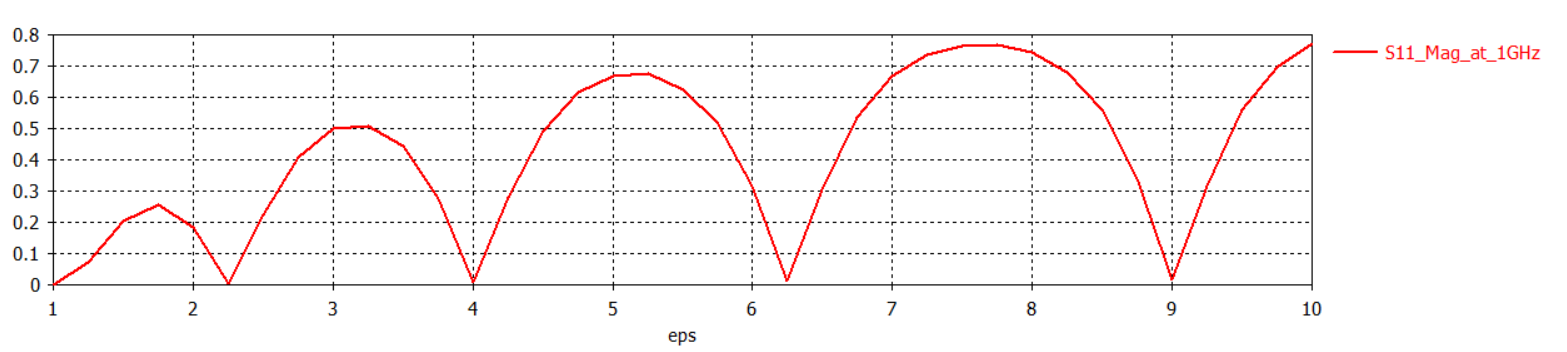
\includegraphics[width=0.91\textwidth]{figures/cst_results/Fig_S11_mag_vs_eps.png}
    \caption{Preserved CST $|S_{11}|$ versus relative permittivity at 1~GHz.}
    \label{fig:s11-mag}
\end{figure}

\begin{table}[H]
\centering
\caption{Selected CST reflection minima preserved in the source report.}
\label{tab:cst-minima}
\begin{tabularx}{\textwidth}{@{}p{0.17\textwidth}p{0.24\textwidth}p{0.24\textwidth}X@{}}
\toprule
\textbf{$\varepsilon_r$} & \textbf{CST $|S_{11}|$} & \textbf{$20\log_{10}|S_{11}|$} & \textbf{Evidence note} \\
\midrule
1.00 & 0.000194892 & -74.20~dB & Preserved sweep value \\
2.25 & 0.00321858 & -49.85~dB & Preserved sweep value \\
4.00 & 0.0104206 & -39.64~dB & Preserved initial validation value \\
6.25 & 0.0128988 & -37.79~dB & Preserved sweep value \\
9.00 & Near zero & Not numerically preserved & Deep minimum visible in sweep plot \\
\bottomrule
\end{tabularx}
\end{table}

The source archive also contains the CST result-table screenshot shown in
Fig.~\ref{fig:result-table}. It provides traceability for the parameterized sweep but
does not replace a raw exported data file.

\begin{figure}[H]
    \centering
    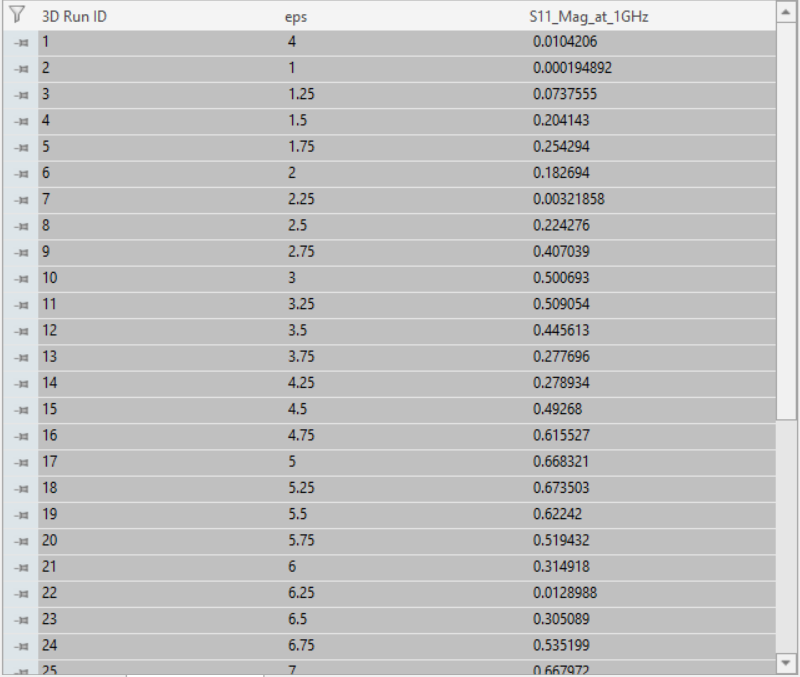
\includegraphics[width=0.72\textwidth]{figures/cst_results/Fig_result_table_s11_mag.png}
    \caption{Preserved CST result table for selected $|S_{11}|$ sweep values.}
    \label{fig:result-table}
\end{figure}

\subsection{Reflection Phase}

The preserved phase response is shown in Fig.~\ref{fig:s11-phase}. Rapid transitions
and wrapping occur near the magnitude minima. This behavior is expected because phase
becomes highly sensitive when the complex reflection coefficient approaches the
origin.

\begin{figure}[H]
    \centering
    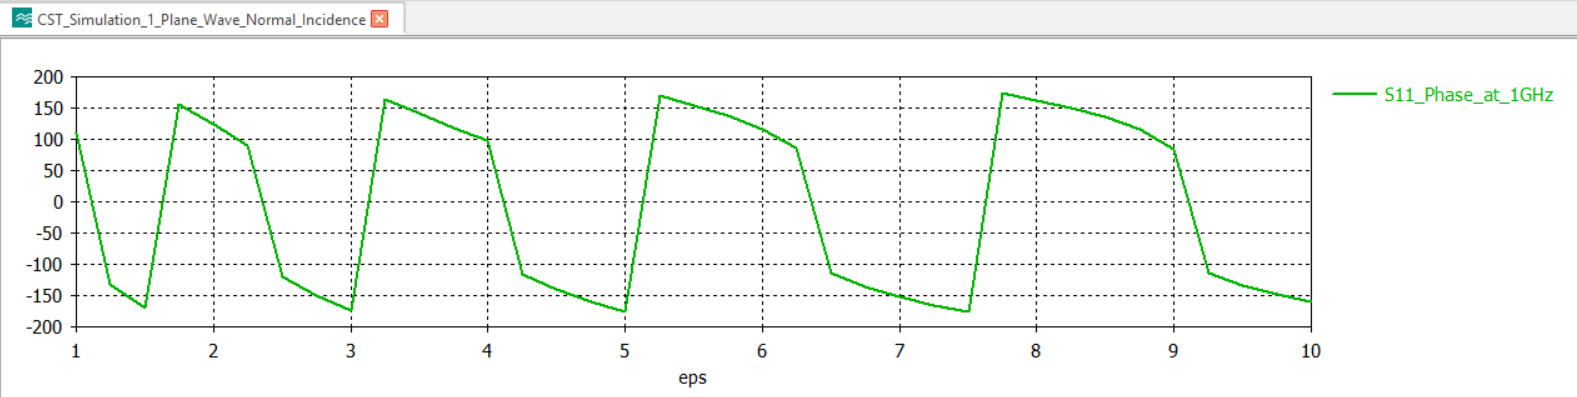
\includegraphics[width=0.91\textwidth]{figures/cst_results/Fig_S11_phase_vs_eps.png}
    \caption{Preserved CST phase of $S_{11}$ at 1~GHz.}
    \label{fig:s11-phase}
\end{figure}

\subsection{Validation Metric}

The primary validation metric is the location of each minimum, not its exact depth.
All five analytically predicted matched permittivity values occur on the 0.25 sweep
grid and are visible as minima in the CST response. Table~\ref{tab:location-comparison}
summarizes this comparison.

\begin{table}[H]
\centering
\caption{Analytical-to-CST comparison of reflection-minimum locations.}
\label{tab:location-comparison}
\begin{tabular}{@{}cccc@{}}
\toprule
\textbf{$m$} & \textbf{Analytical $\varepsilon_r$} & \textbf{CST minimum location} & \textbf{Location difference} \\
\midrule
2 & 1.00 & 1.00 & 0.00 \\
3 & 2.25 & 2.25 & 0.00 \\
4 & 4.00 & 4.00 & 0.00 \\
5 & 6.25 & 6.25 & 0.00 \\
6 & 9.00 & 9.00 & 0.00 \\
\bottomrule
\end{tabular}
\end{table}

The zero location differences reflect the fact that the analytical matched values
coincide exactly with sampled sweep points. They do not establish that the CST null
depths have converged to the ideal analytical zeros.
